\chapter{System Interaction Diagrams}

% This chapter requires a good 1-2 pages
% prefacing the way systems will behave
% and introducing the types of diagrams
% that will be shown.

\section{Introduction}
PLACEHOLDER TEXT --REPLACE WITH OUR OWN INTRO--

The following is an analysis of the interaction of UC-1 to
UC-5.  Within these use cases we touch on two of the most
integral parts of our system, the persistant database, and
the Yahoo! Finanace API adapter. The diagrams clearly describe
the interactions of different subsystems to satisfy the use
cases intent. Beyond the afformentioned subsystems, other
subsystems are introduced 

\iffalse

Following is an analysis of the interactions of the two most
important internal subsystems in our system as identified in
our domain model, the financial data retrieval subsystem and
the asynchronous processing subsystem. The interaction diagrams
included clearly describe the interactions that occur within
each of these subsystems. They elaborate upon the mechanics
behind our use cases, but do not necessarily correspond to them
one-to-one. This is because several of our use cases are
completely facilitated through the browser and controller to
generate views for the users, and as such it would not be
interesting or worthwhile to explore the internal interactions.
The following analysis clearly describes how market orders are
placed and processes, how information is retrieved from Yahoo!
Finance, and how we manage asynchronous processes (i.e. a queue)
in order to process market orders and enact our mailer system.
\fi

\section{Diagrams}

\begin{figure}[H]
\centering
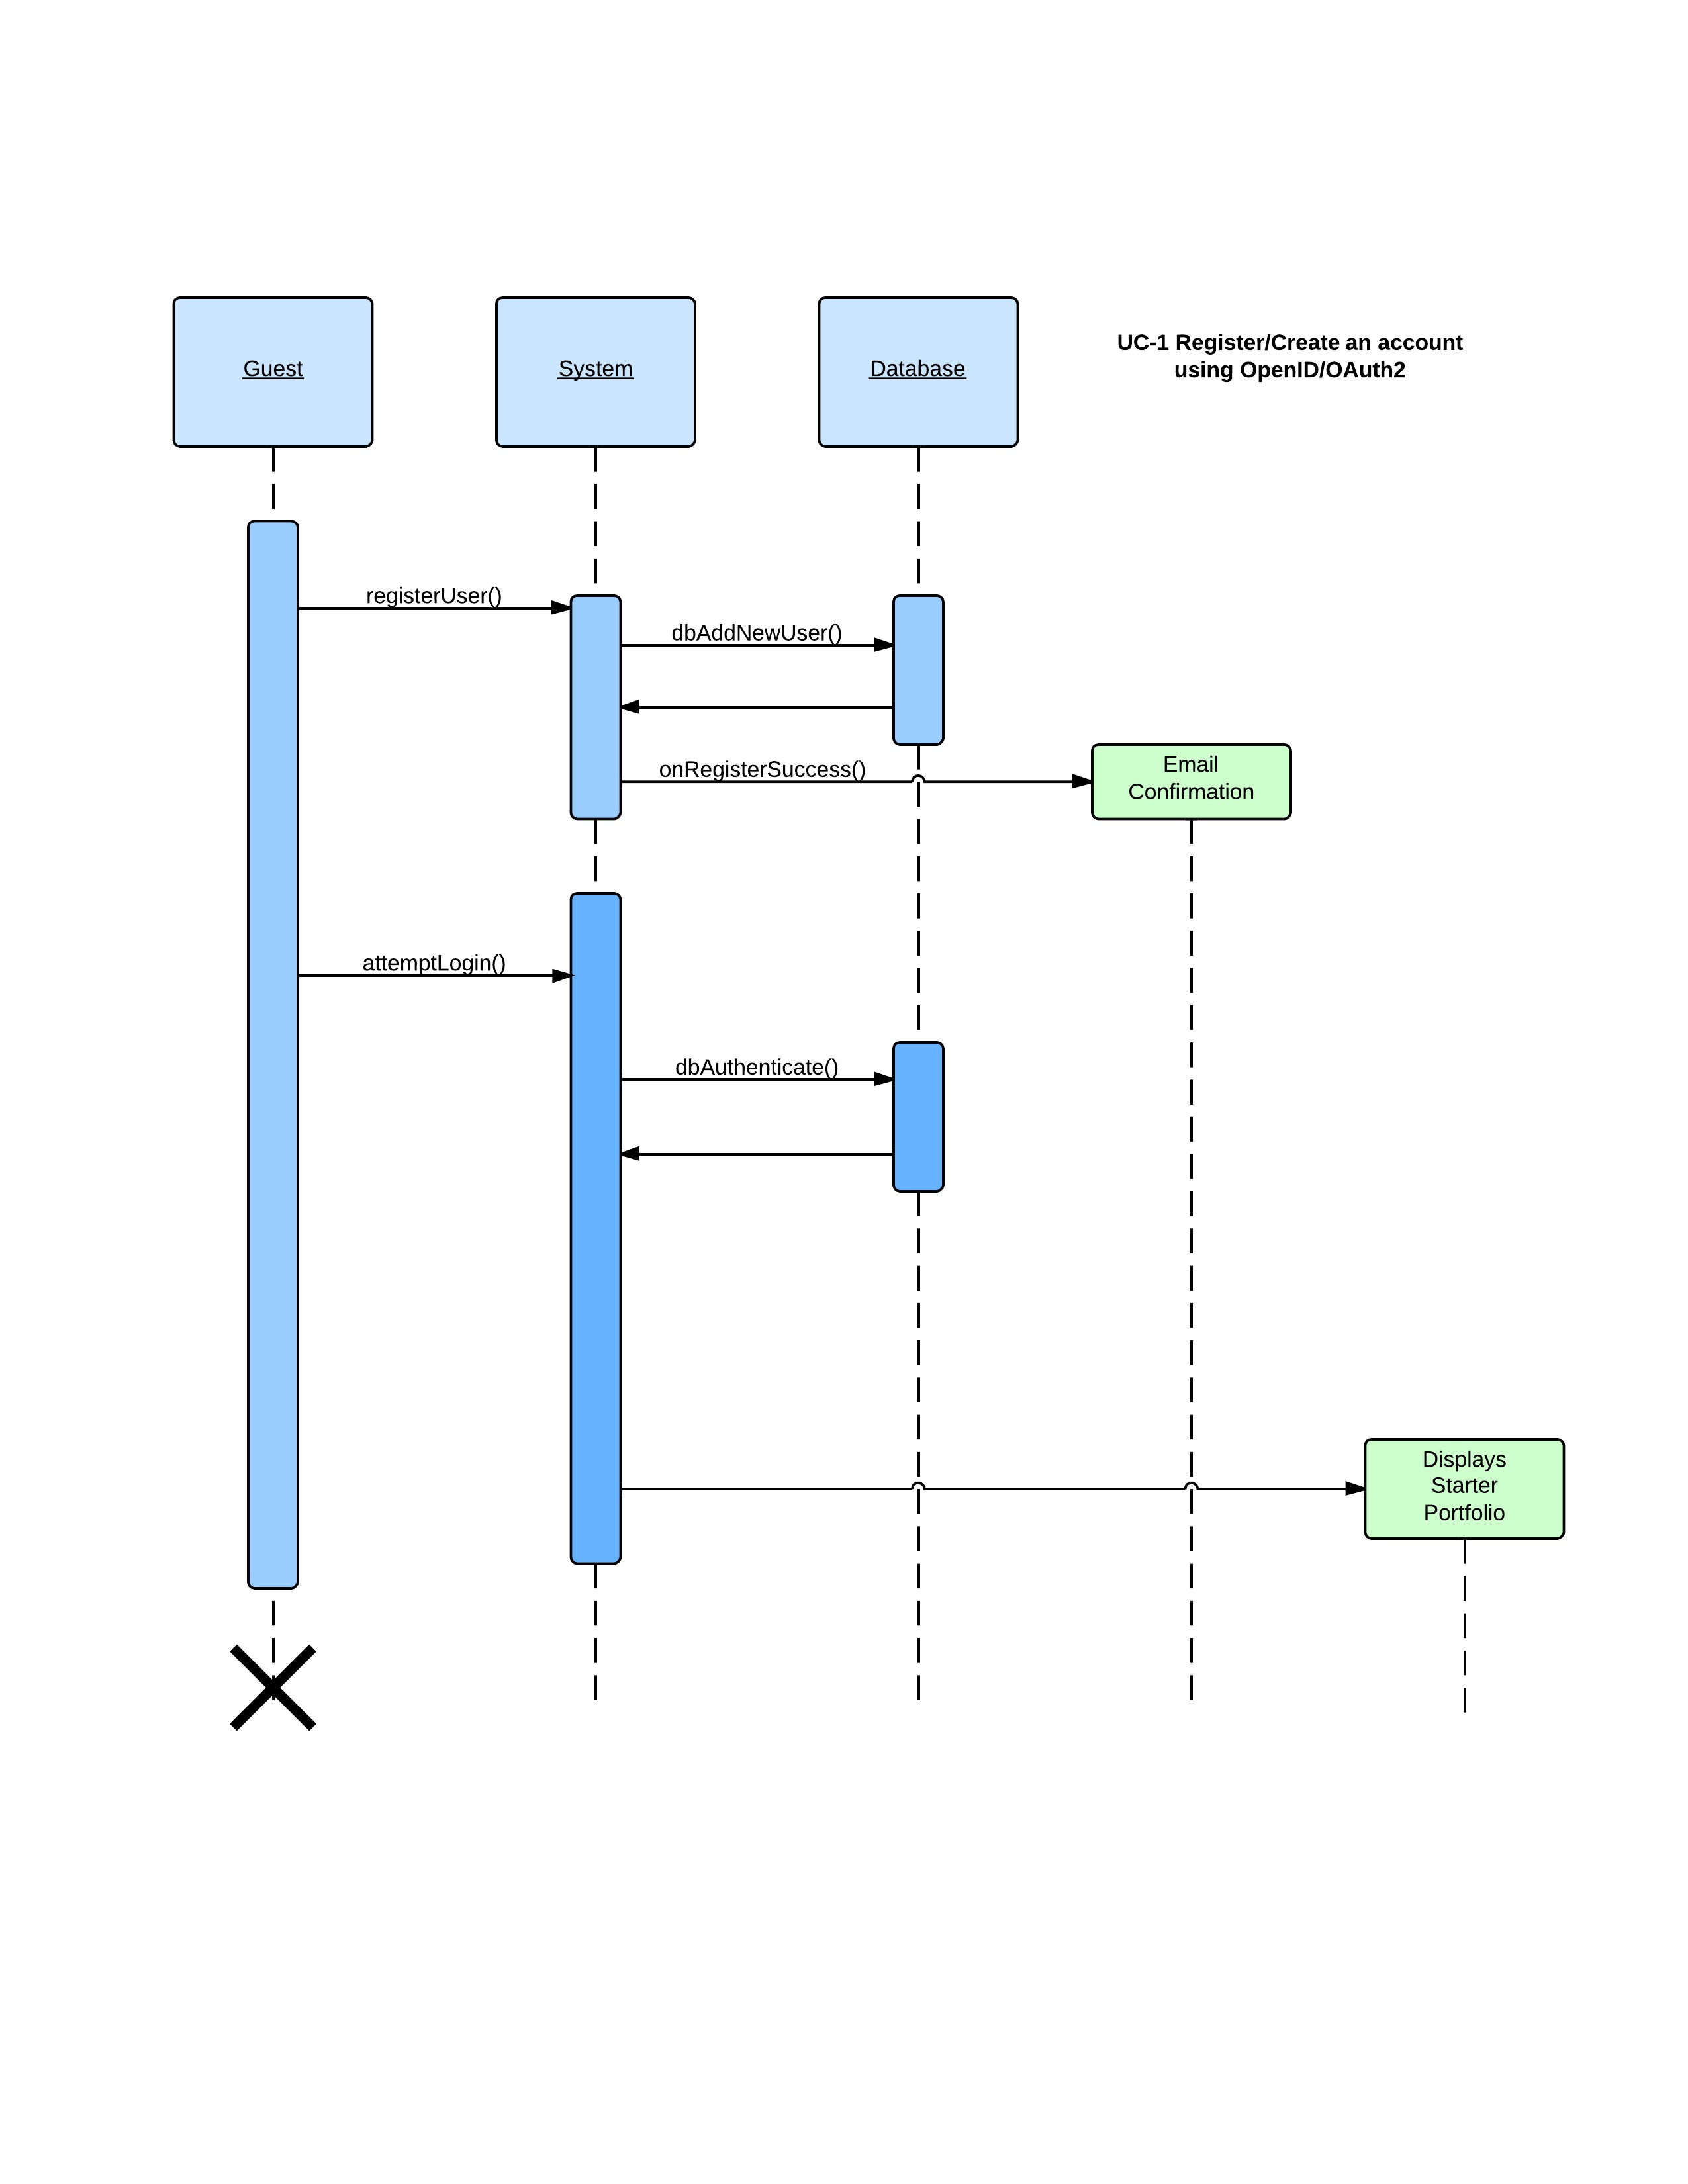
\includegraphics[width=5.5in]{./img/inter/uc1.jpg}
\caption{Shown in the sequence diagram
for UC-1 begins with two options for the Guest. Either login or
register an account. If a user attempts to register a new account
the system is contacted with the user’s information. Then the
system can attempt to check to make sure no duplicate login
information exists in the database and if not it will store the new
user information into the database. After this happens the user will
be sent a confirmation email. If a user attempts to login, the system will
attempt to authenticate
the login details with details found in the database. If the details
match correctly then the system will send the guest into investor
mode and continue to upload their portfolio setting.}
\end{figure}



\begin{figure}[H]
\centering
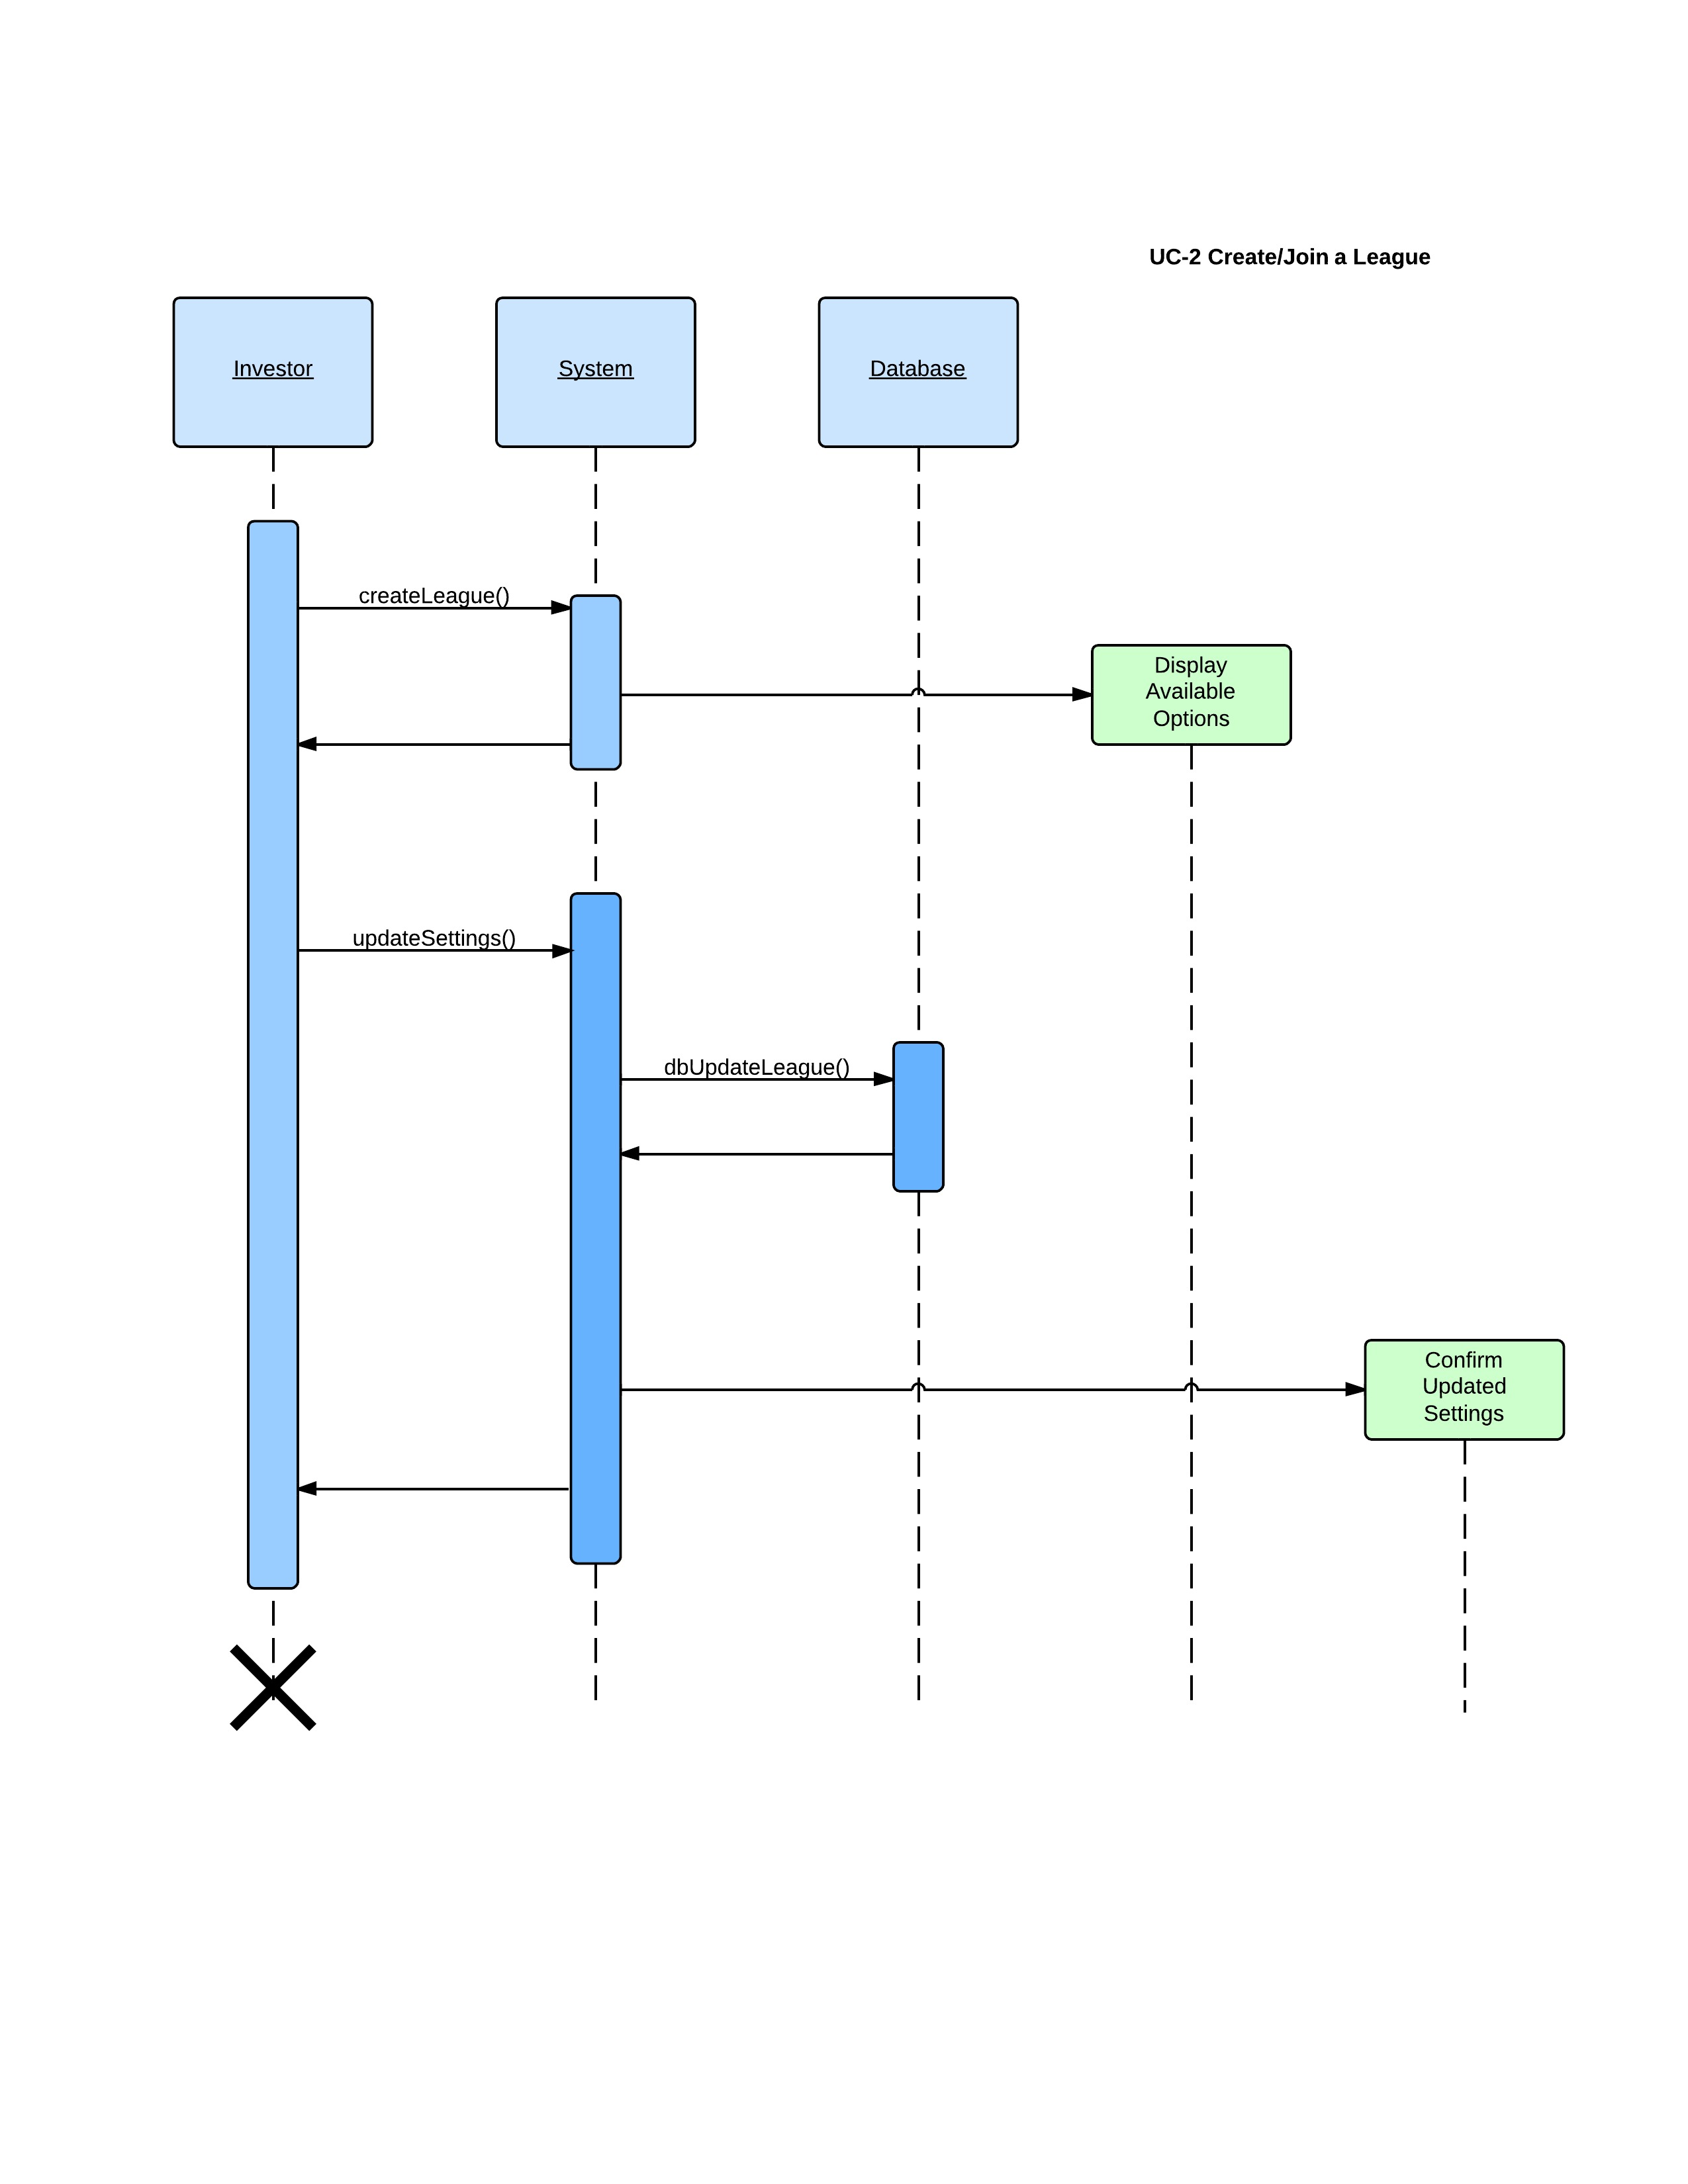
\includegraphics[width=5.5in]{./img/inter/uc2.jpg}
\caption
{\iffalse See UC-2 on page \pageref{UC-2}.\fi Shown in the sequence diagram for
UC-2 is the flow of how to create an investment league. When an
investor selects to create a league the system and more specifically
the league controller will be contacted. The system will display
the available options for creating a league. After there is a function
updateSettings() which will create the league and process it in the
database and also allow settings to be updated for a league. Not
shown in the diagram is the alternative case of joining a league.
The process to join a league is straightforward, where the league
controller will show available leagues and then if an investor
chooses to join they will be entered into the list in the database
to associate with this league.}
\end{figure}



\begin{figure}[H]
\centering
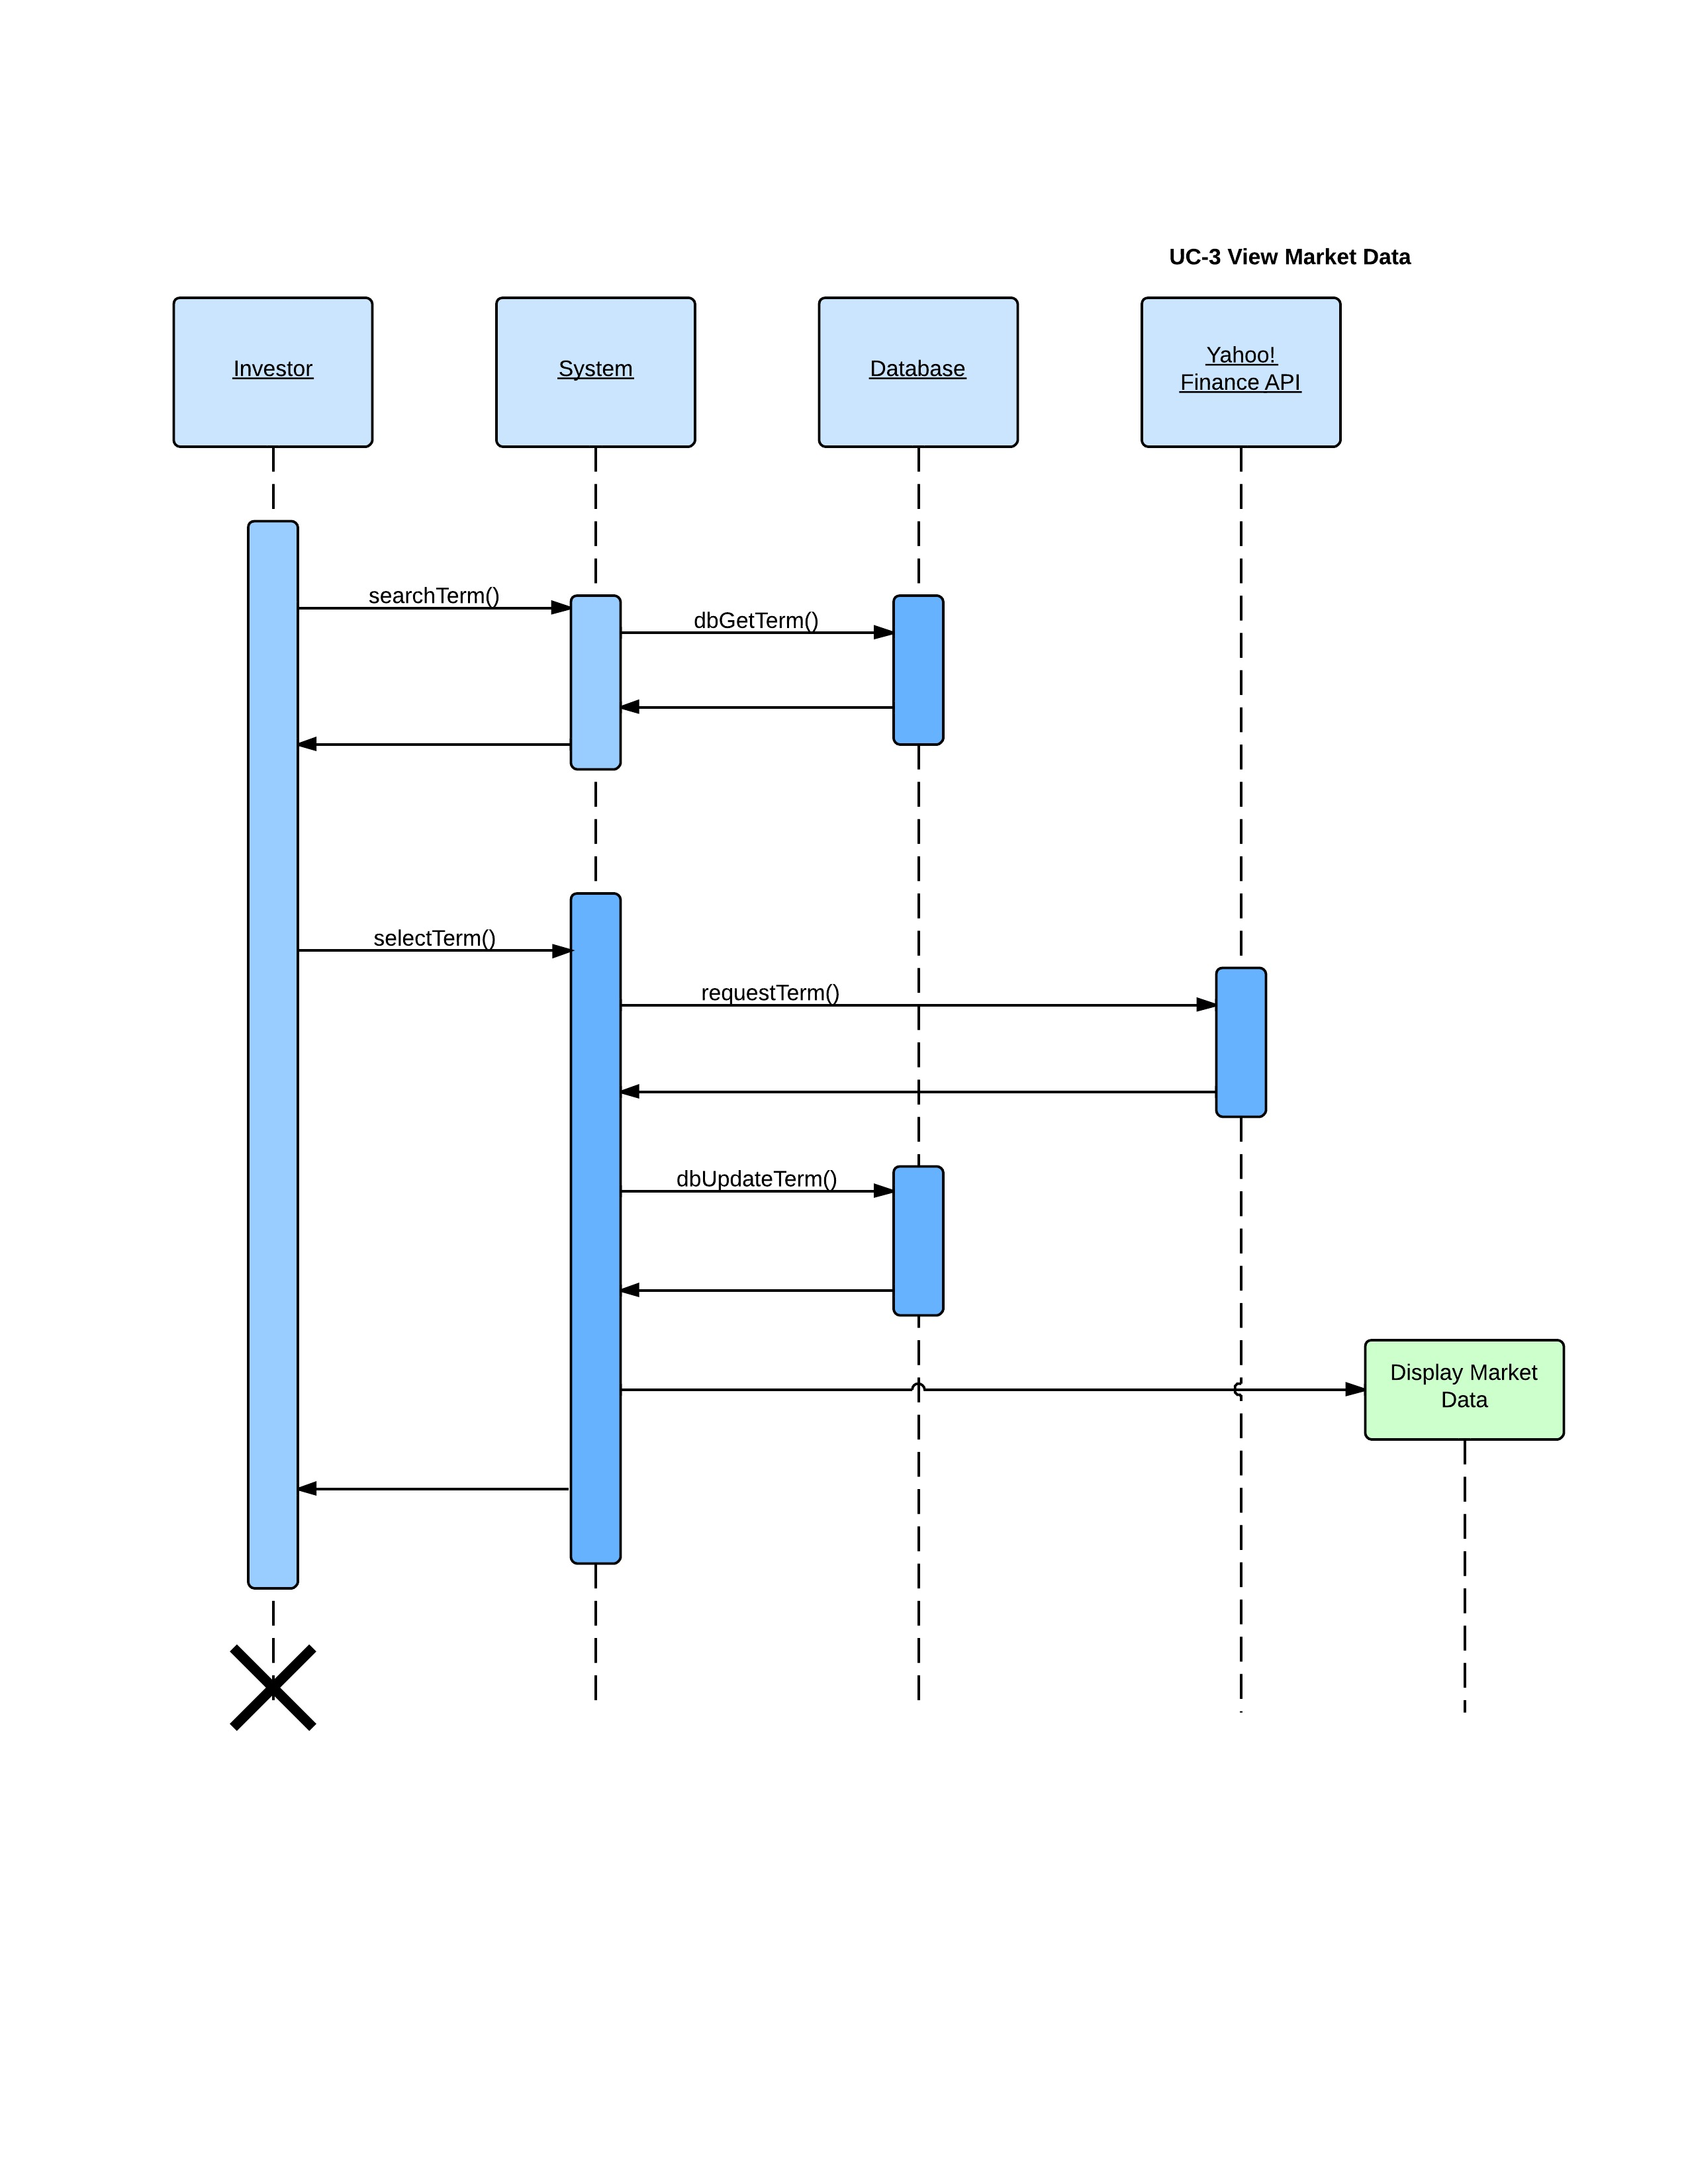
\includegraphics[width=5.5in]{./img/inter/uc3.jpg}
\caption
{\iffalse See UC-3 on page \pageref{UC-3}.\fi Viewing market data is accomplished by
an investor searching a term. The system then finds this term which is
most likely a company name or stock symbol. The system will fetch matches
from the database and display them from the user. The investor will choose
a match. The system takes the chosen term and requests its data from the
Yahoo! Finance API. The system will update the database for this term, and
then continue to display its market data to the investor.}
\end{figure}



\begin{figure}[H]
\centering
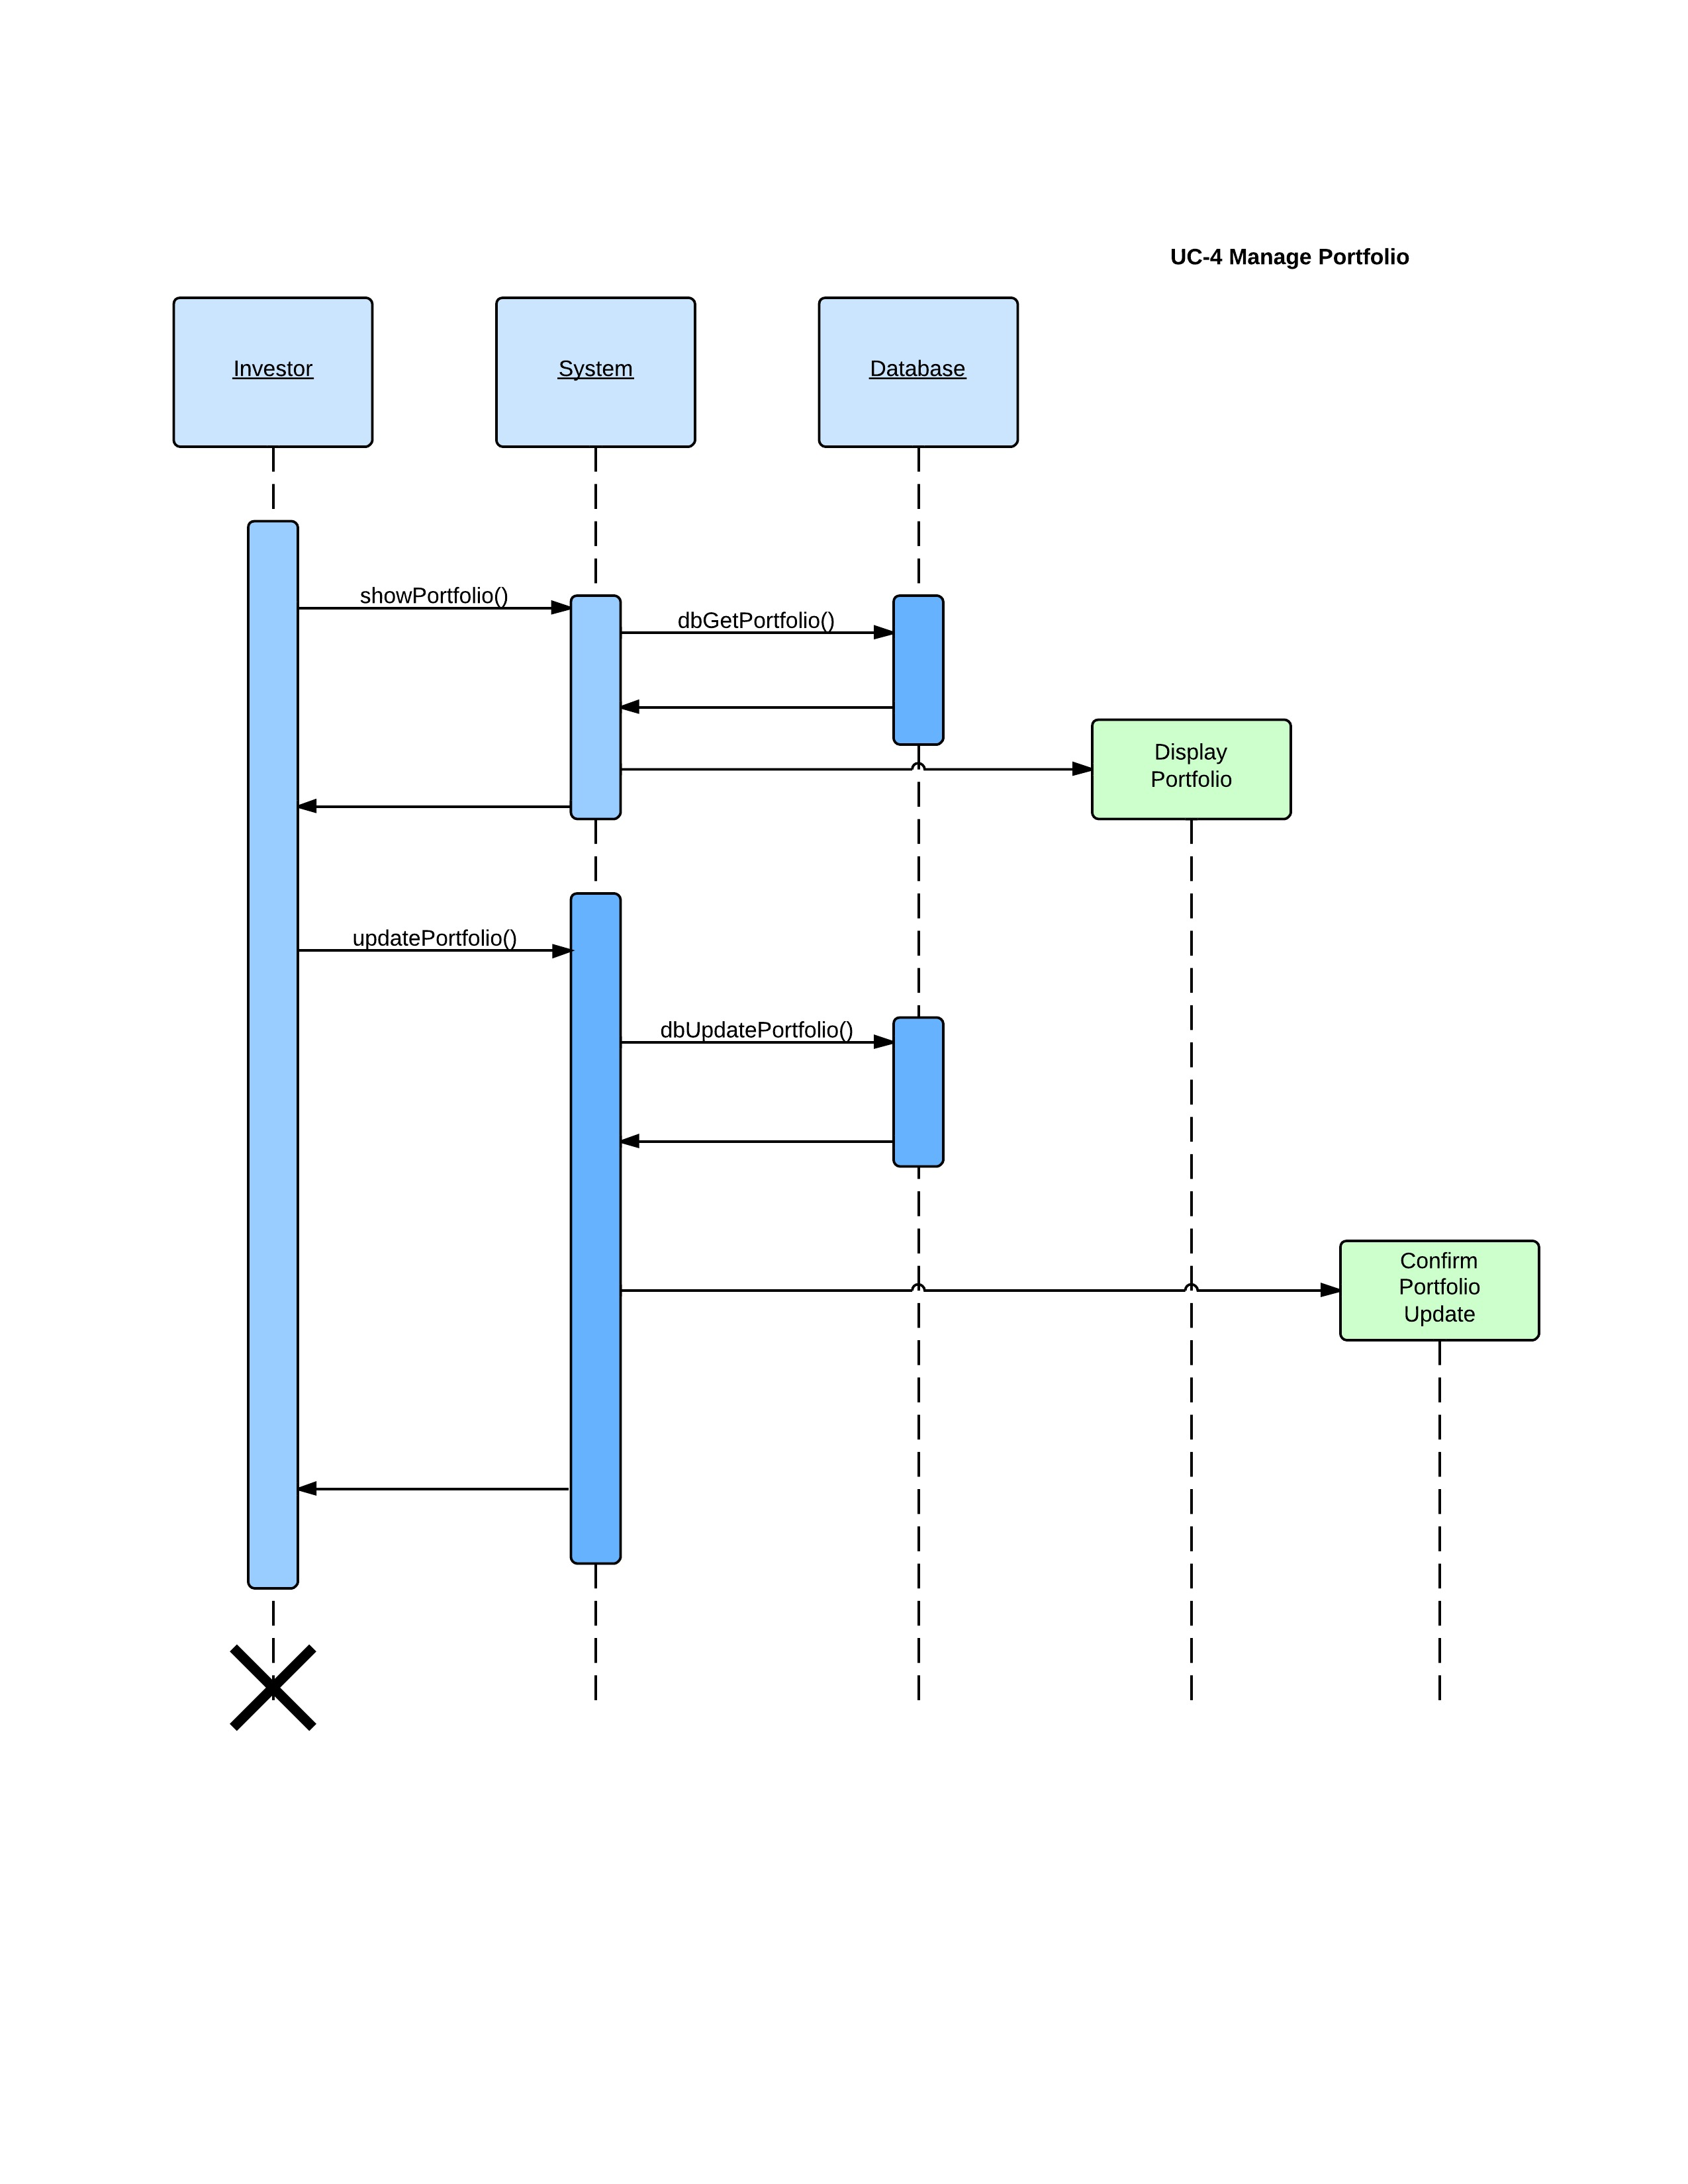
\includegraphics[width=5.5in]{./img/inter/uc4.jpg}
\caption
{\iffalse See UC-4 on page \pageref{UC-4}.\fi The investor should be able to view and
make changes to their portfolio. The investor should be able to view their
portfolio. The system will fetch the investor’s portfolio stocks from the
database. The investor can also update their view of the portfolio and other
settings.}
\end{figure}



\begin{figure}[H]
\centering
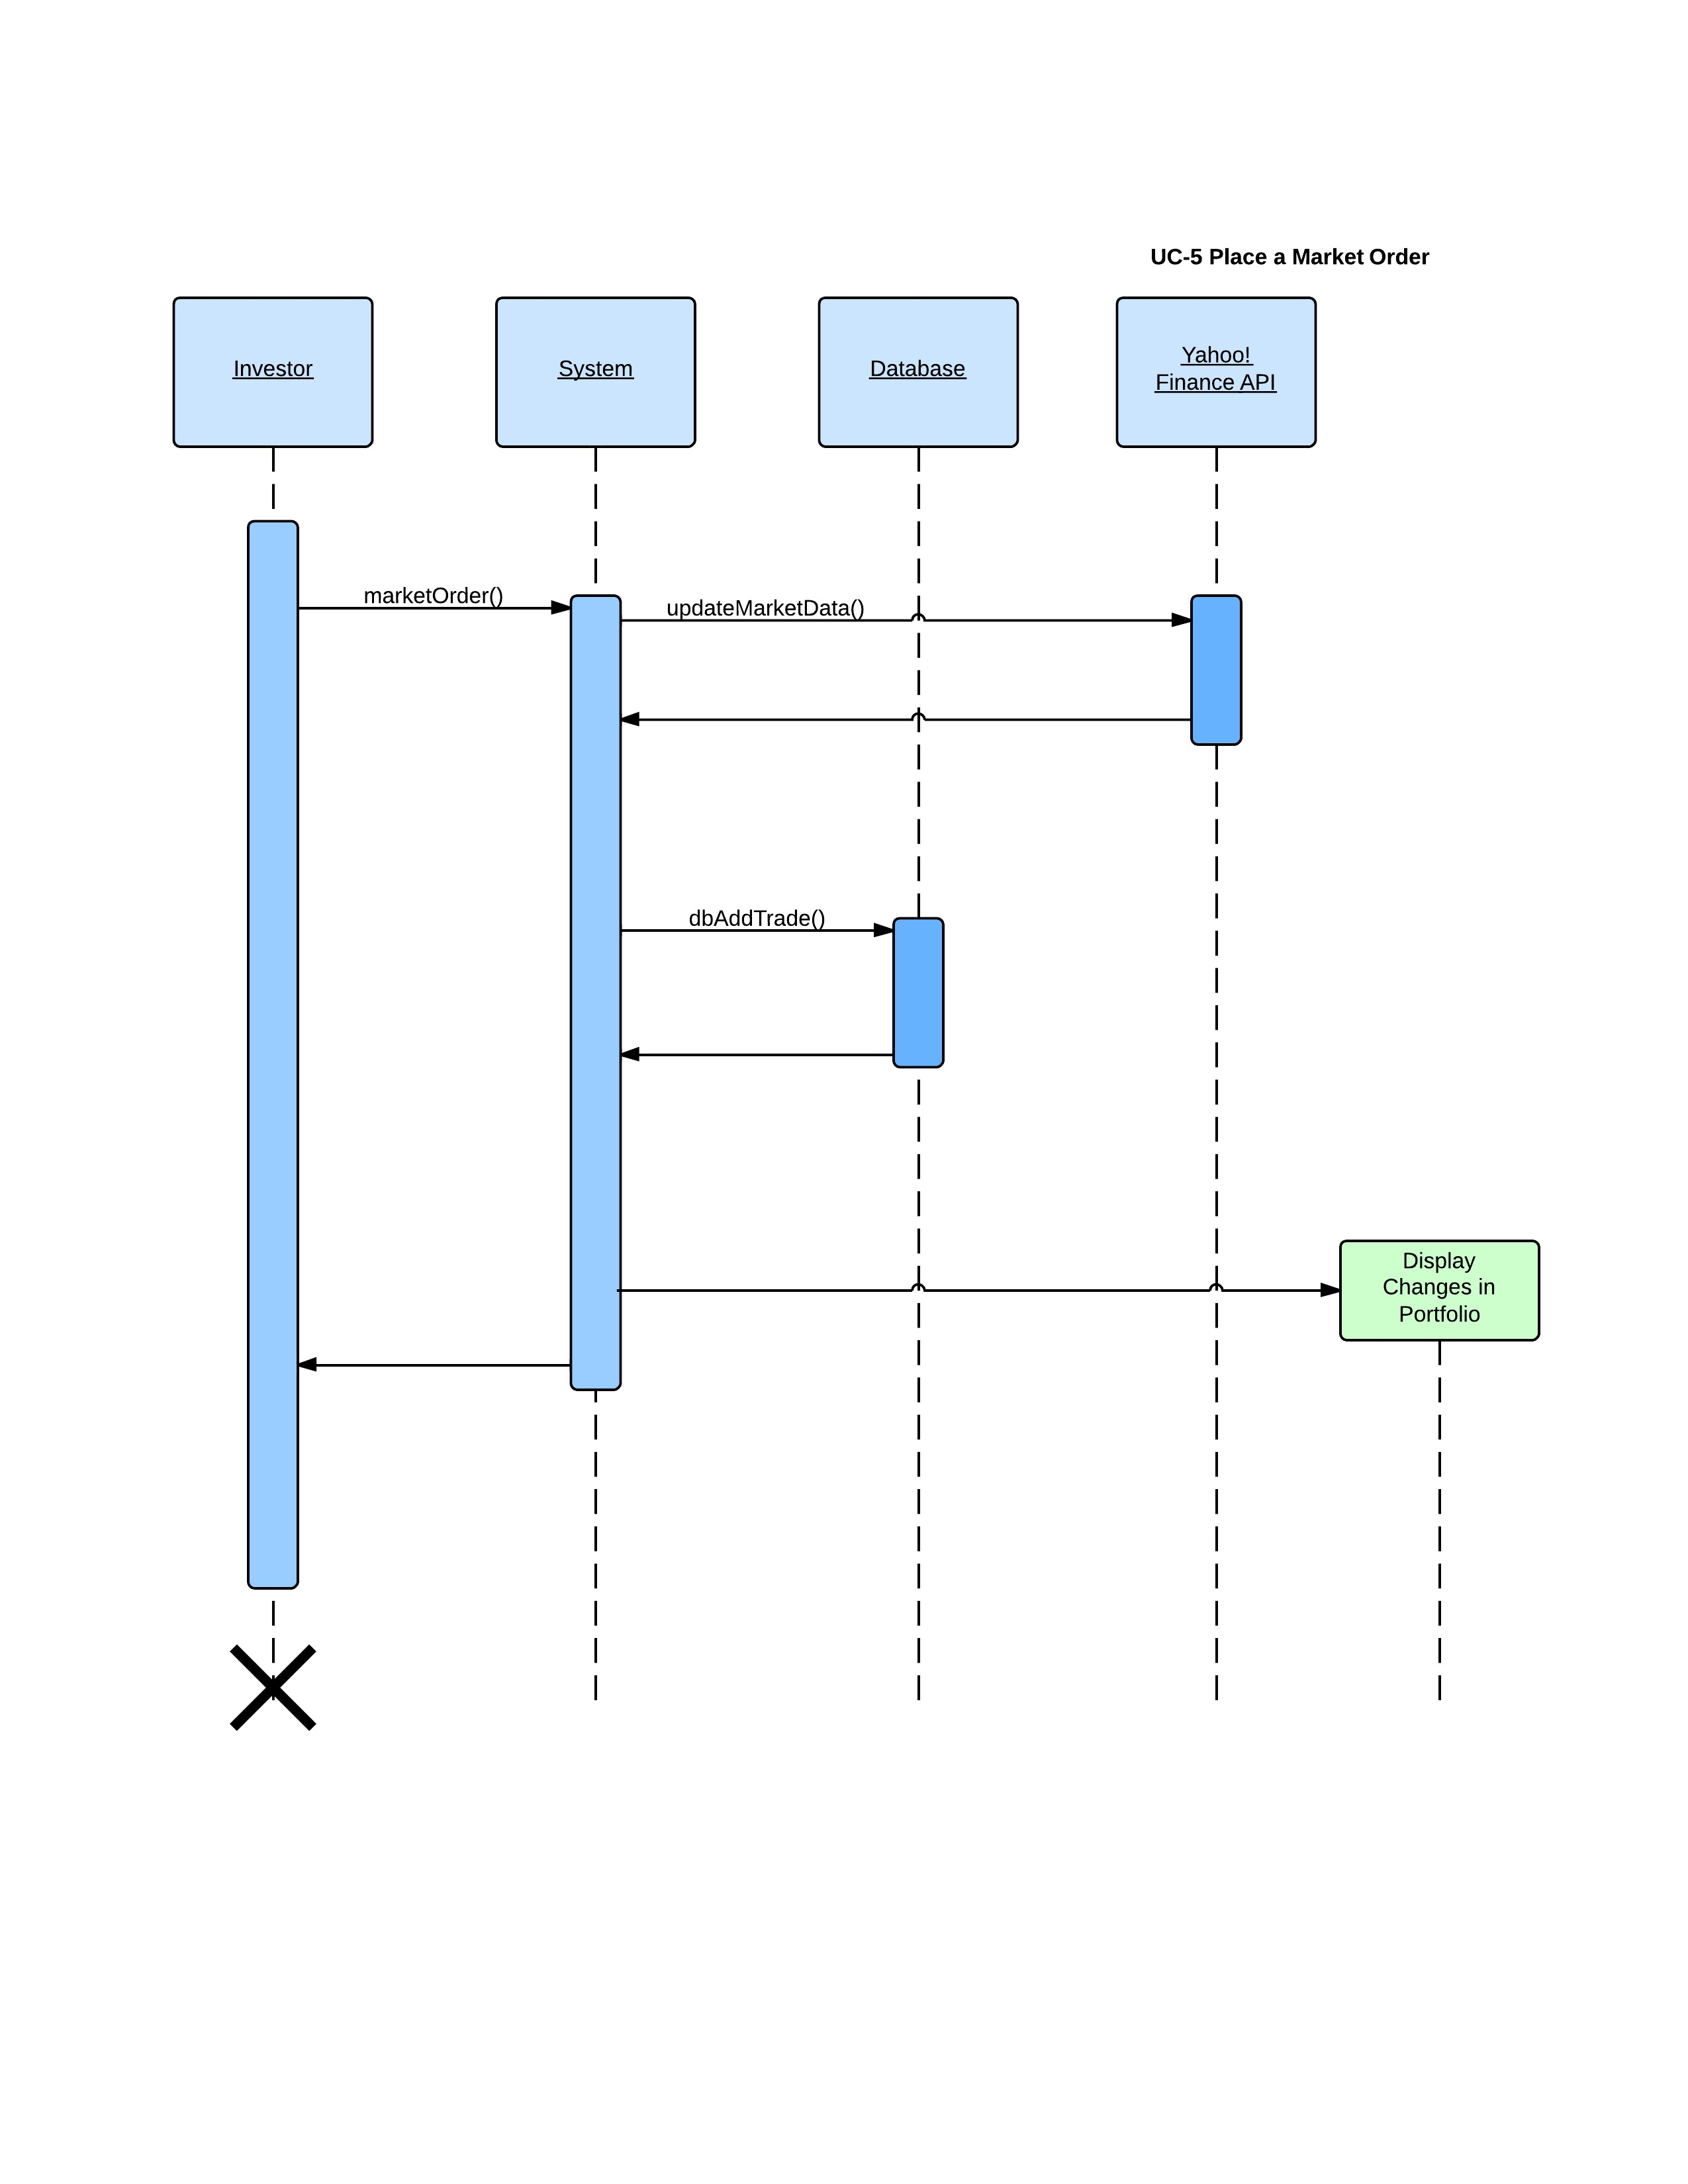
\includegraphics[width=5.5in]{./img/inter/uc5.jpg}
\caption
{\iffalse See UC-5 on page \pageref{UC-5}.\fi The investor needs to be able to place market
orders. As soon as the investor places an order the system contacts Yahoo!
Finance API to retrieve the current price of the stock. After the current price
is found the system must confirm with the database that the user has enough funds
to make a buy offer or enough stock to make the sell offer. After the trade is
confirmed information will be stored about it in the database and the changes
will be displayed in the investor’s portfolio.}
\end{figure}



